% Chapter Template

\chapter{Experimento: Buscando el Efecto Espejo en una tarea Perceptual} % Main chapter title

\label{Cap_Exp} % Change X to a consecutive number; for referencing this chapter elsewhere, use \ref{ChapterX}

%----------------------------------------------------------------------------------------
%	SECTION 1
%----------------------------------------------------------------------------------------
\section{Planteamiento general}

%Se propone buscar evidencia del Efecto Espejo en una tarea fuera de Memoria de reconocimiento


%Se propone una tarea perceptual ya que carece de una fase de preparacion
El interés principal del trabajo aquí expuesto es evaluar la posibilidad de que el Efecto Espejo y los patrones de respuesta identificados como parte del mismo, sean un producto del uso del modelo de detección de señales en la comparación del desempeño de los participantes a lo largo de dos condiciones de dificultad cualesquiera y no así de una discrepancia en el grado en que se tratan dichas condiciones a nivel de ciertos procesos superiores de atención y memoria alterando el orden en que dichos estímulos se distribuyen en el eje de la evidencia. Para ello se diseñó una tarea de detección meramente perceptual, donde las condiciones de dificultad fueron construidas con base en su discriminabilidad perceptual.\\ 

%Se trabaja con ilusiones opticas, dado que la literatura en ellas permite anticiparnos a la d' y proponer dos niveles de dificultad.
Las ilusiones ópticas 

\subsection{Objetivo}

%Buscar evidencia del efecto espejo en una tarea de detección que no implique el reconocimiento de estimulos ya conocidos.
Poner a prueba la existencia de los patrones de respuesta identificados como parte del Efecto Espejo en una tarea de detección perceptual con dos niveles de dificultad, (i.e. una tarea de detección que no pertenezca a la familia de tareas de reconocimiento y, principalmente, que carezca de una etapa previa a la fase experimental donde los participantes tuvieran ocasión de manipular los estímulos y dar un trato distinto a cada nivel de dificultad).\\

\section{Construcción de los Experimentos}

Para poner a prueba la extensión del Efecto Espejo a fenómenos más allá de la memoria de reconocimiento, se diseñó una tarea de detección perceptual donde el objetivo de los participantes era señalar aquellos ensayos en que dos círculos a comparar fueran del mismo tamaño, indicando si éste era el caso ensayo a ensayo presionando una de dos posibles teclas.\\ 

La ilusión de Ebbinghaus (a.k.a. Círculos de Titchner) refiere a un fallo en la estimación del tamaño de un círculo cuando este aparece rodeado por un halo de círculos uniformes de mayor o menor tamaño (Ver Figura~\ref{fig:Ebbinghaus}). La ilusión suele ser explicada como resultado de la interferencia provocada por la estructura de los estímulos sobre el sistema cognoscitivo-perceptual que evalúa 

\begin{figure}[th]
\centering

\includegraphics[width=0.55\textwidth]{Figures/Ebbinghaus} 
\decoRule
\caption[Ilusión de Ebbinghaus ejemplar]{Ilustración de la Ilusión de Ebbinghaus. Los círculos centrales de ambas figuras son del mismo tamaño. Sin embargo, el círculo central de la figura izquierda tiende a ser percibido como más pequeño (efecto de subestimación) y el círculo derecho suele ser percibido como más grande (efecto de sobrestimación), como producto del contraste que guardan con los círculos circundantes.}
\label{fig:Ebbinghaus}
\end{figure}

De acuerdo a \parencite{Massaro1971}, la

\subsection{Estímulos}

\begin{itemize}
\item Experimento 1 : Circulo de referencia aislado vs Figura de Ebbinghaus.

Los estímulos utilizados en el Experimento 1 se diseñaron de acuerdo a un diseño factorial de 5x2x2, (Ver Figura~\ref{fig:Exp_1}). 
 

\item Experimento 2 : Figura de Ebbinghaus (Sobrestimación) vs Figura de Ebbinghaus (Subestimación).
\end{itemize}



\begin{figure}[th]
\centering
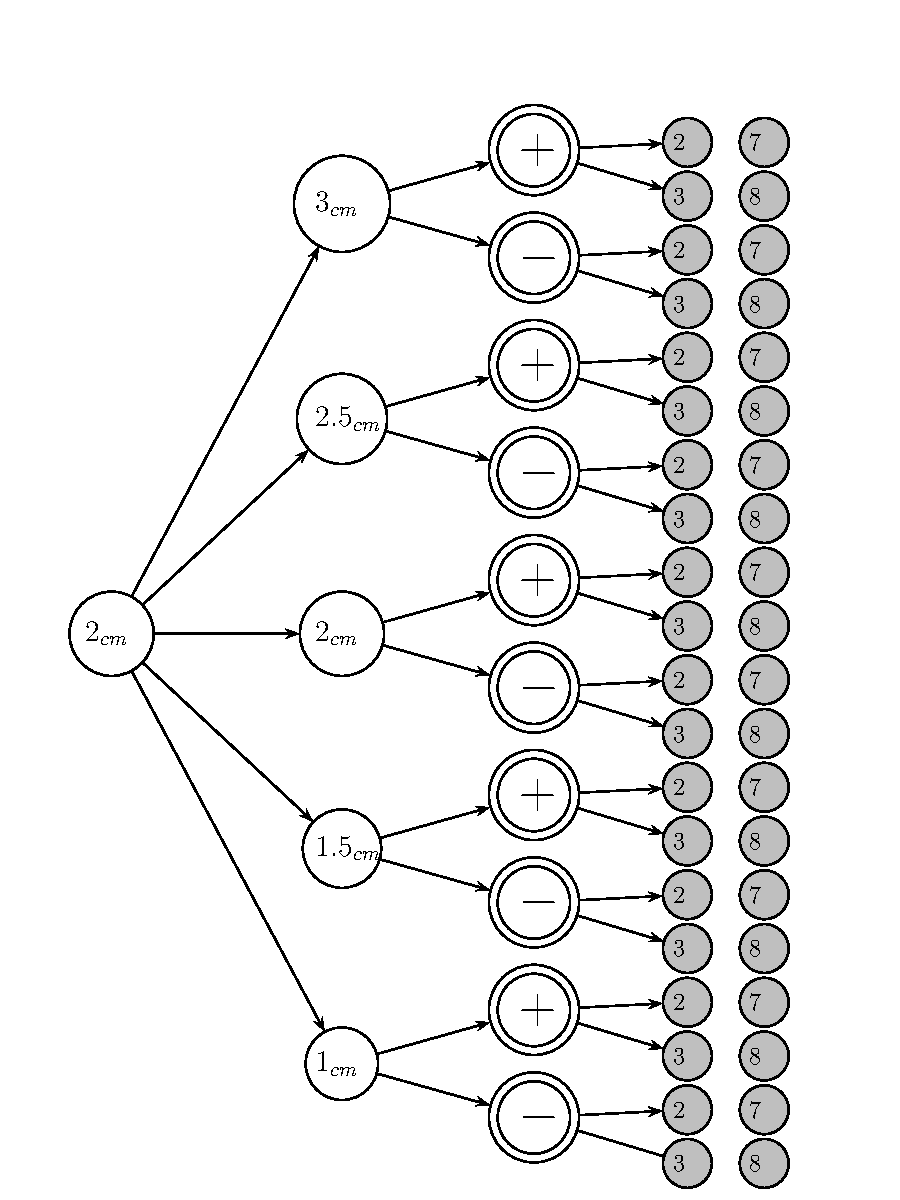
\includegraphics[width=0.99\textwidth]{Figures/Estimulos_Experimento1} 
\decoRule
\caption[Diseño de Estimulos en el Experimento 1]{Diseño factorial (5x2x2) utilizado para construir los estímulos utilizados durante la tarea de detección en el Experimento 1. En cada ensayo los participantes tenían que comparar el tamaño de un círculo de referencia constante con el círculo central de una figura de Ebbinghaus, que podía aparecer en cinco posibles tamaños, con círculos externos que inducen efectos de sobrestimación o subestimación (indicado en el esquema con  y signos positivos y negativos, respectivamente) y con dos niveles de 'número de círculos externo' por condición (2 y 3 círculos externos en la condición fácil o 7 y 8 en la condición difícil). Por cada condición de dificultad, se tienen 16 estímulos con ruido, (10 repeticiones por cada uno, en cinco colores diferentes) y 4 que contienen la señal (repetidos 40 veces cada una, en cinco colores diferentes), dejándonos con 320 ensayos por condición y un total de 640 ensayos en el experimento.}
\label{fig:Exp_1}
\end{figure}


\begin{figure}[th]
\centering
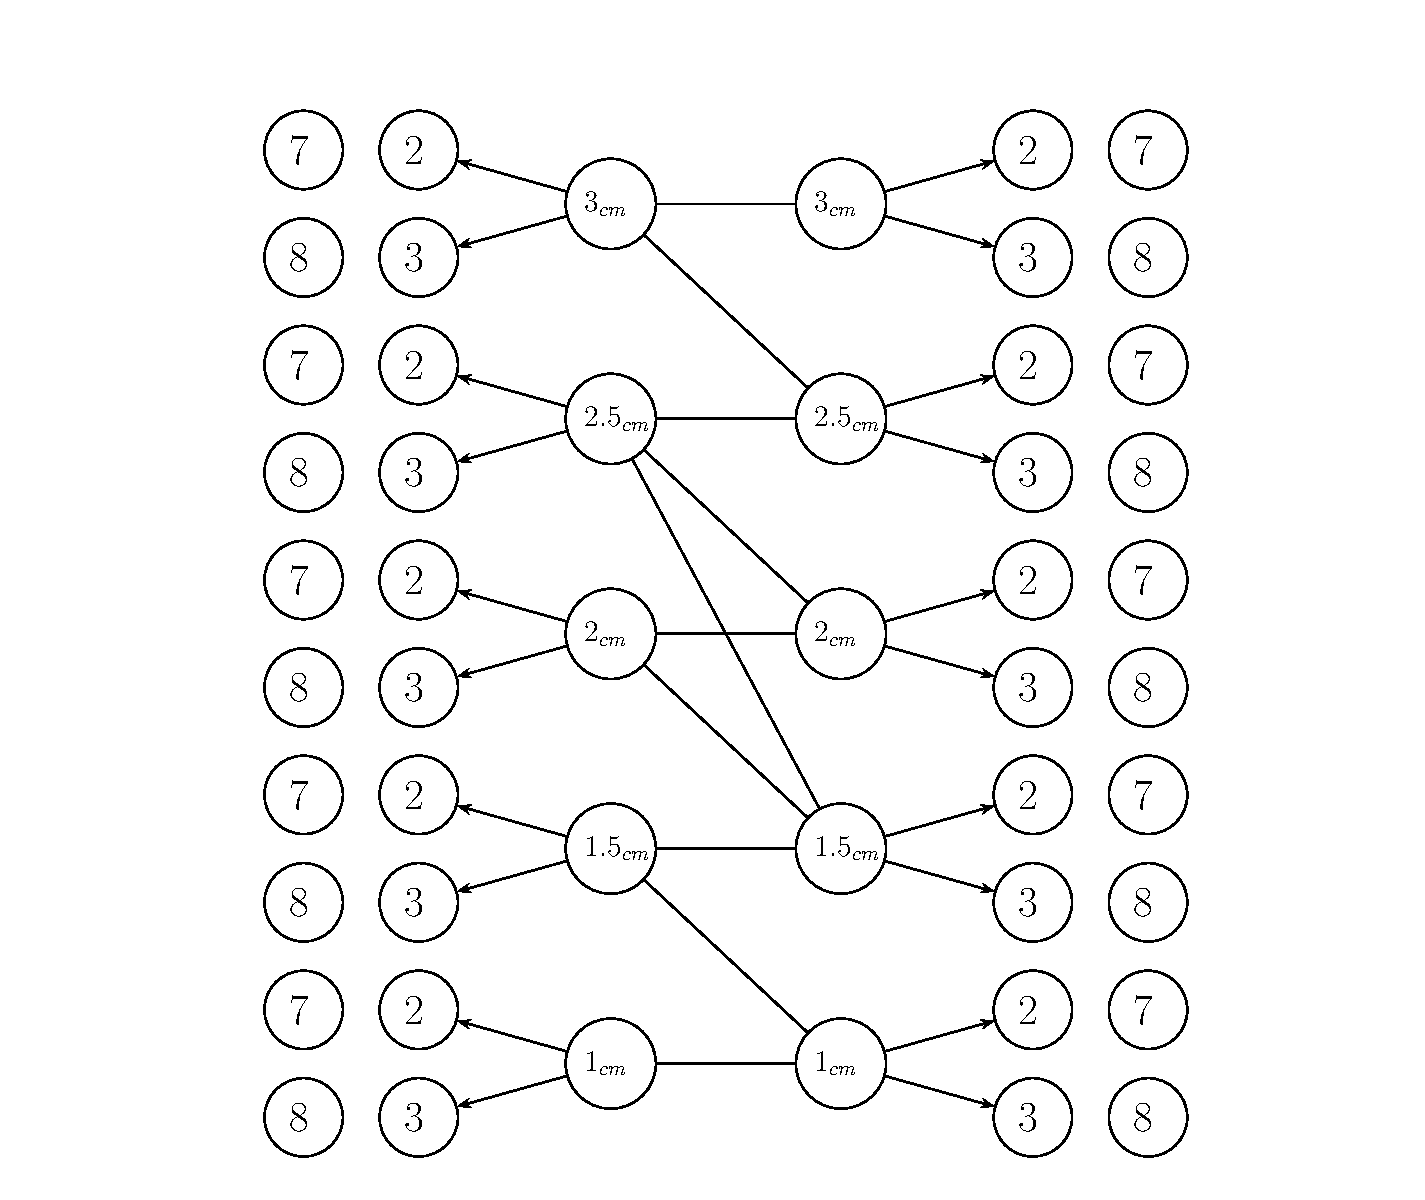
\includegraphics[width=0.99\textwidth]{Figures/Estimulos_Experimento2} 
\decoRule
\caption[Diseño de Estimulos en el Experimento 2]{Diseño de las parejas  de figuras de Ebbinghaus a comparar en el Experimento 2. Se manejaron cinco tamaños distintos de círculo central, que se mostraron en parejas iguales (cinco señales) y cinco parejas desiguales (cuatro cuyos círculos centrales diferían en 0.5 cm y, una con una diferencia de 1 cm). En cada pareja siempre había una figura de Ebbinghaus que inducía la subestimación del tamaño central y una que promovía la subestimación, contrabalanceando el orden en que aparecían en pantalla (relativo a la posición izquierda o derecha). Por cada pareja de círculos centrales, se contemplaron cuatro combinaciones posibles entre los dos niveles de círculos externos contenidos por cada condición (i.e. a vs a, b vs b, a vs b, b vs a; donde a y b son sustituíbles por 2 y 3 círculos externos en la condición fácil o 7 y 8, en la condición difícil.)}
\label{fig:Exp_2}
\end{figure}


\subsection{Materiales}

La tarea fue programada y ejecutada en la plataforma Psychopy v.12 para Python.  

\subsection{Participantes}

Un total de cuarenta y un estudiantes de la Facultad de Psicología participaron en alguno de los dos experimentos. Los 

 el Experimento 1 se llevó a cabo con veinte participantes y el Experimento 2, con veintiuno. Ambos experimentos se llevaron a cabo simultáneamente por lo que la asignación de los participantes a cualquiera de los mismos se hizo de manera alternada, procurando garantizar que la muestra de parti

\section{Procedimiento}

Se controló que la distancia que separase los estímulos presentados se encontrara dentro de un ángulo de $X grados$ del campo visual de los participantes, así como que estos realizaran la tarea en una distancia de 1 m respecto del monitor.

\subsection{Registro de respuestas}

El experimento fue programado de manera tal que por cada participante se obtuviera un documento en formato csv (i.e. comma separated value) que contuviera información, ensayo a ensayo, sobre la respuesta dada por 
